\section{Design implementation using Lua scripting language}
After working with libreCAD 3, I experimented with it by making some designs usign Lua scripting language.
\noindent In this project, I made  several lua scripts and run it in LibreCAD to make various design. I made design of water tank and varoius logos and some other impressive 2D design in LibreCAD using LUA scripting language. 
In LibreCAD v3, there is a dockable window for creating lua scipts:
\begin{figure}[!ht]
\centering
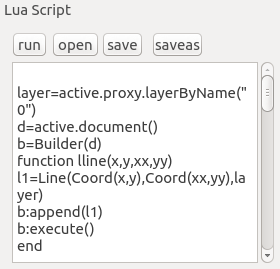
\includegraphics[scale=0.7]{images/lualogo/lua.png}                   
\vspace{-1em}
\caption{Lua Dockable window }
\hspace{-1.5em}
\end{figure}
\begin{figure}
\begin{center}
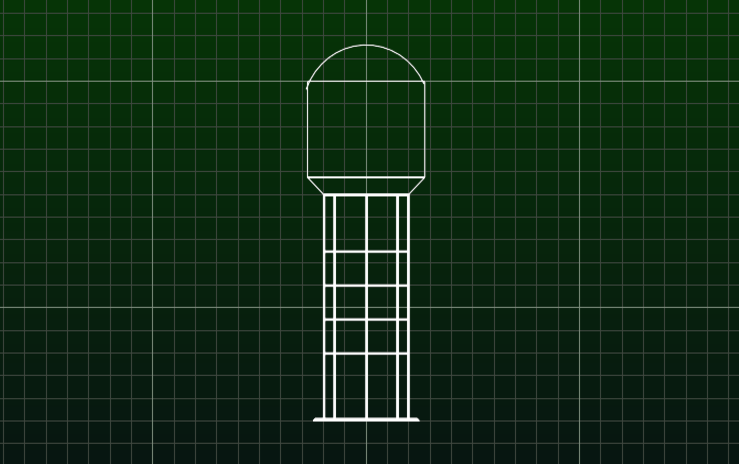
\includegraphics[scale=0.5]{images/lualogo/w2.png}
\caption{Water Tank Model}

\includegraphics[scale=0.4]{images/lualogo/xmen.png} 
\caption{X-Men Logo}
%
\includegraphics[scale=0.4]{images/lualogo/chakra1.png}
%\caption{Sharp Design 1}

\includegraphics[scale=0.4]{images/lualogo/chakra2.png}
\caption{Sharp Design 2}
\end{center}
\end{figure}
